\documentclass[11pt]{beamer}
\usetheme[progressbar=frametitle]{metropolis}
\usepackage[utf8]{inputenc}
\usepackage[spanish]{babel}
\usepackage{fancyvrb}
\definecolor{new_green}{HTML}{347F1F}


\author{Lic. Agustina Pesce \\ Lic. Santiago Soler}
\title[Taller de {\LaTeX}]{Taller Introductorio a {\LaTeX}: \\ Cómo producir documentos de Calidad}
\subtitle{Segundo Encuentro: Artículo Científico}
%\setbeamercovered{transparent} 
%\setbeamertemplate{navigation symbols}{} 
%\logo{} 
%\institute{} 
\date{}
%\subject{} 

\begin{document}
\maketitle

\section{El Articulo Científico}

\begin{frame}{Estructura Básica de un Artículo Científico}
 \begin{itemize}[<+- | alert@+>] % Con esto hacemos que aparezcan los items de a uno
  \item Título
  \item Autores
  \item Abstract (resumen)
  \item Cuerpo (secciones y subsecciones)
 \end{itemize}
\end{frame}

\section{¿Cómo se hace en \LaTeX{}?}

\begin{frame}[fragile]{Artículo Científico}
 \textbf{Ejemplos de un articulo en \LaTeX{}}
 \begin{columns}
  \column{0.6\textwidth}
  {\color{new_green}
  \begin{Verbatim}[fontsize=\scriptsize]
   \documentclass[a4paper,12pt]{article}
   \usepackage[utf8]{inputenc}
   
   \title{Acá coloco el título del documento}
   \author{El nombre del/los autor/es}
   
   \begin{document}
   \maketitle
   
   \begin{abstract}
    Con este entorno creo
    el resumen del trabajo.
   \end{abstract}

   \section{Nombre de la 1ra Sección}
   Acá empiezo a escribir mi trabajo.
   \subsection{Nonbre de la Subsección}
   \end{document}
  \end{Verbatim}
  }
   \hfill
   \column{0.4\textwidth}
   {\scriptsize
   Declaro el tipo de documento, papel y tamaño de letra. 
   Defino la codificación del documento. \\
   \vspace{2.5em}
   Defino el título. \\
   Defino el autor. \\
   \vspace{2.5em}
   Creo el título y el autor \\
   \vspace{2.5em}
   Creo el Abstract \\
   \vspace{2em}
   Creo una sección y una subsección.
   Usando $*$ no se numera la sección.
   \vspace{4.5em}
   }
 \end{columns}
\end{frame}

\begin{frame}{Artículo Científico}
 \begin{center}
 Veamos un ejemplo...
 \end{center}
\end{frame}

% \begin{frame}{Artículo Científico}
%  Después de compilar:
%  \vspace{-1em}
%  \begin{figure}[b]
%   \centering
%   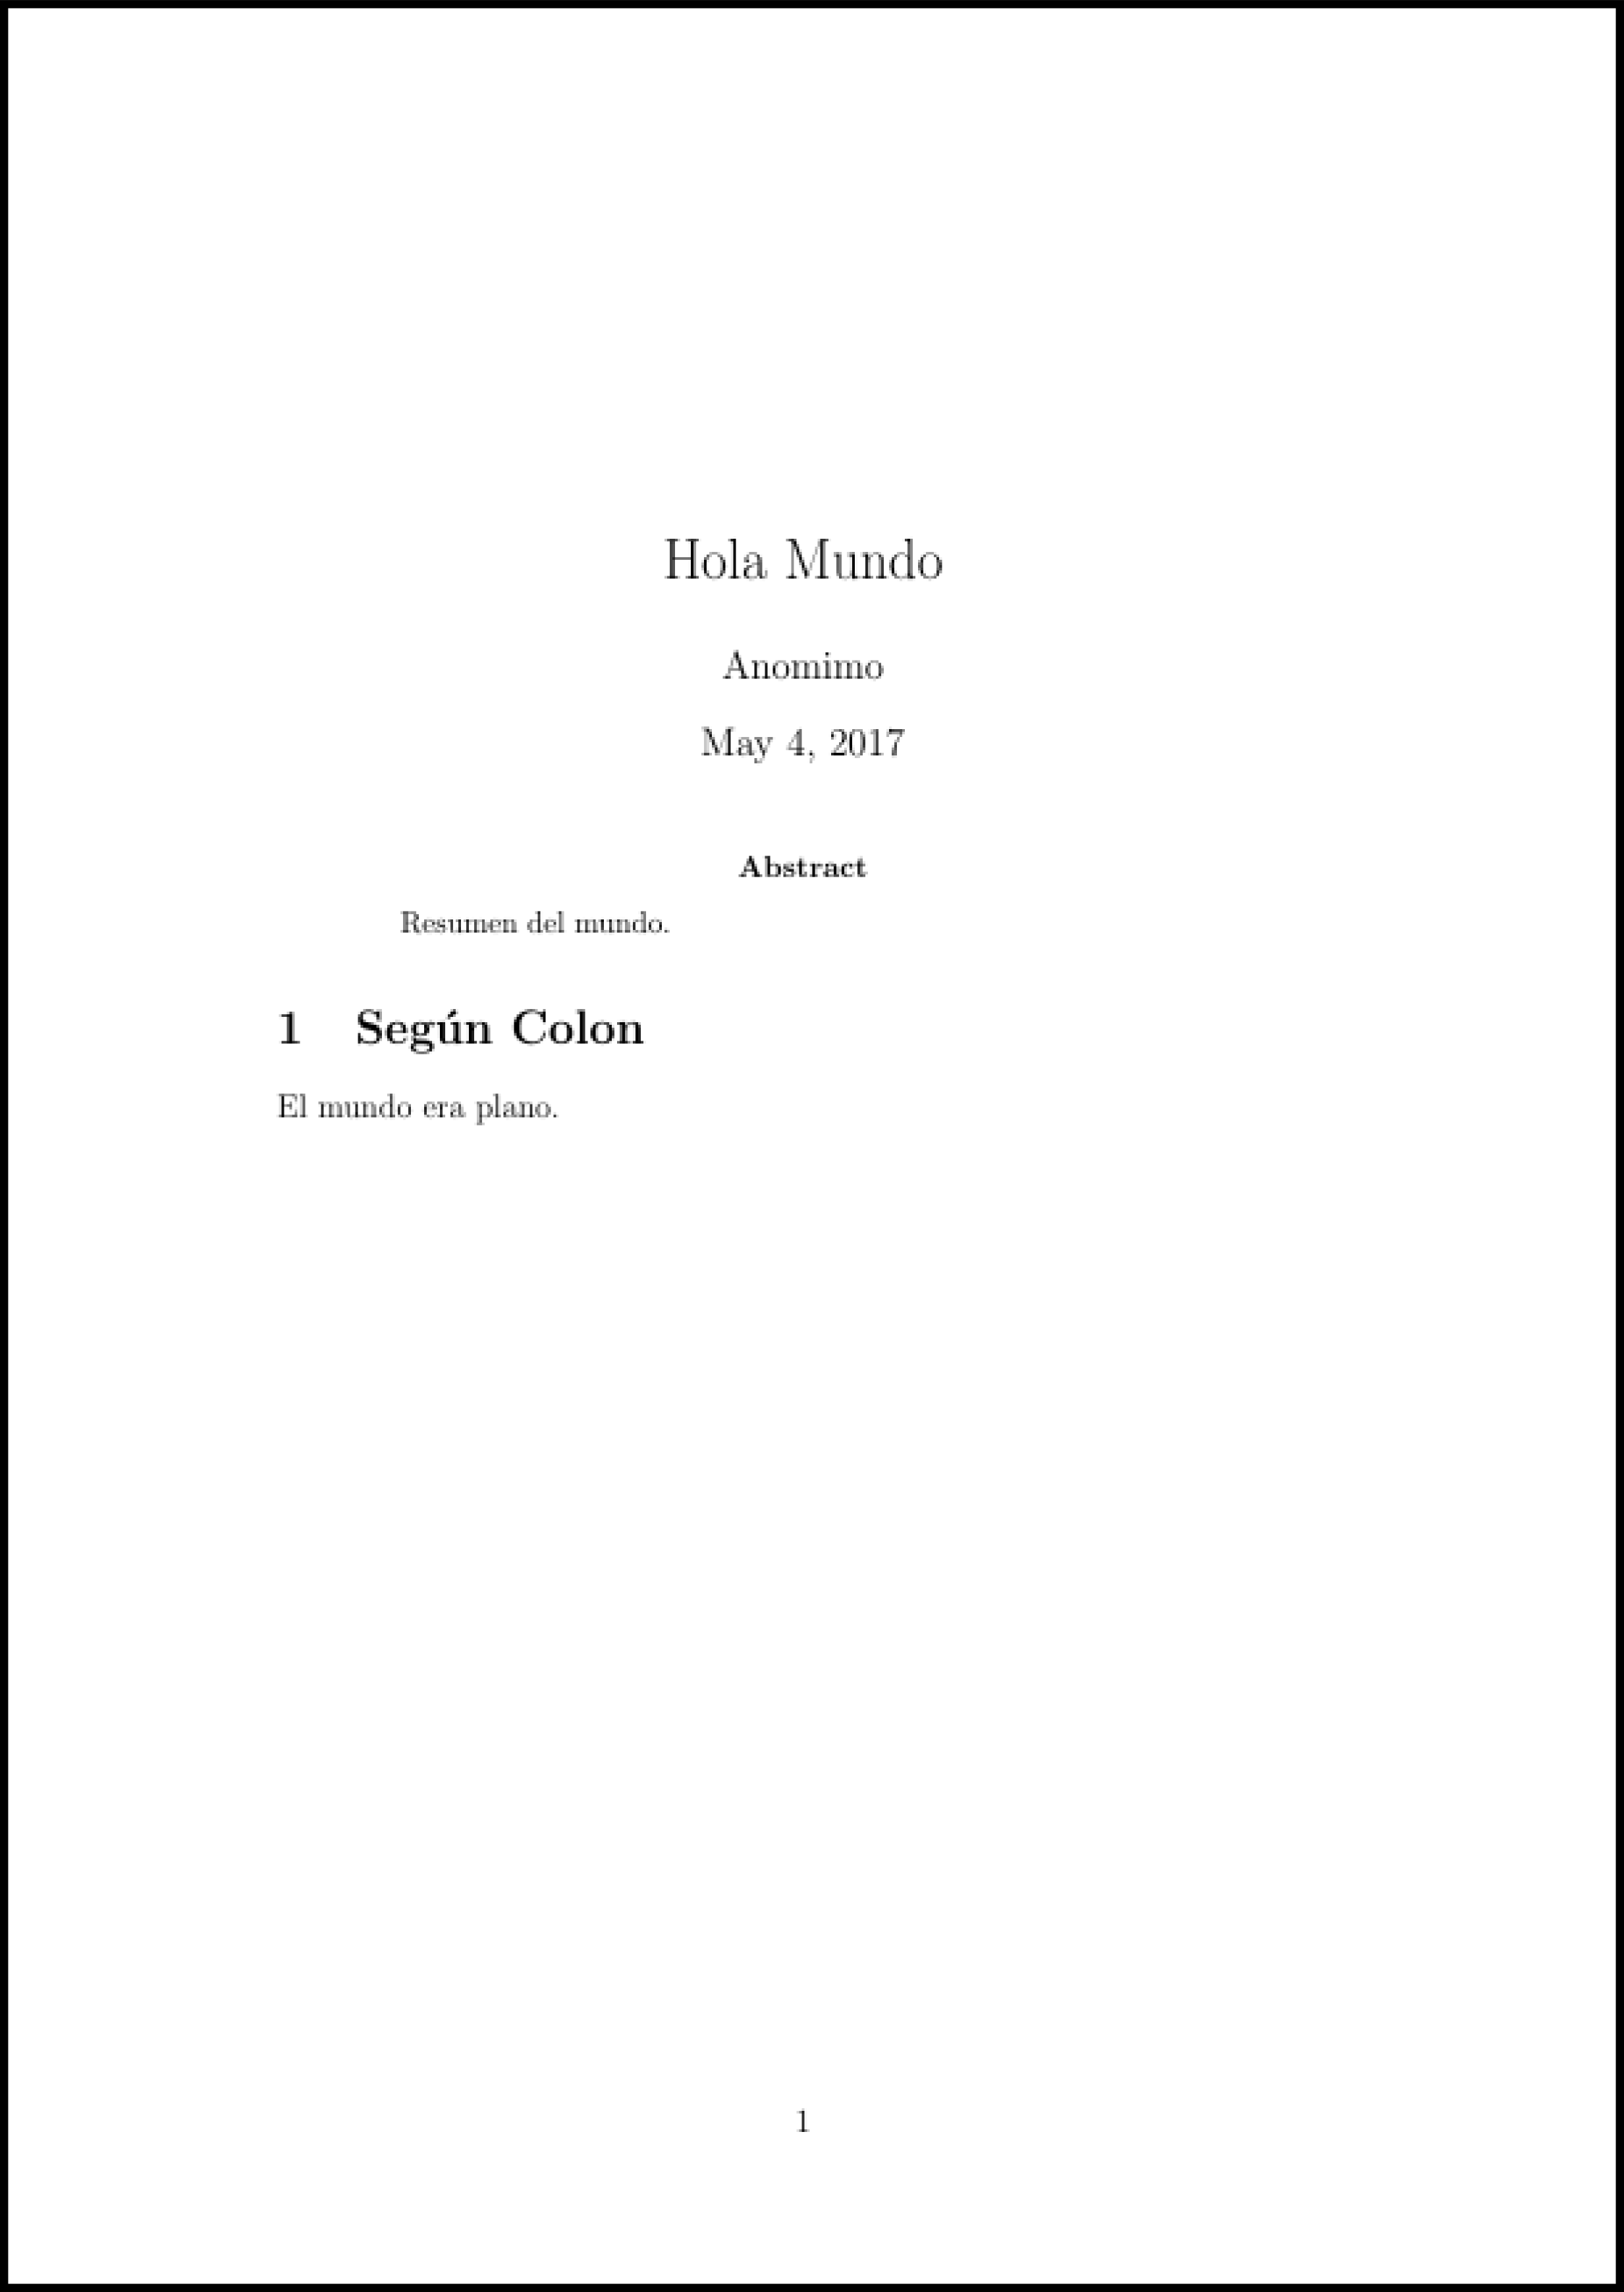
\includegraphics[width=0.45\textwidth]{figs/ej1.png}
%  \end{figure}
% \end{frame}

\begin{frame}{Artículo Científico}
 \begin{center}
 Su turno de hacerlo...
 \end{center}
\end{frame}

\begin{frame}{Artículo Científico}
 \begin{center}
  ¿Qué más necesito para hacer un articulo?
 \end{center}
\end{frame}

\begin{frame}{Artículo Científico}
 \begin{itemize}[<+- | alert@+>] % Con esto hacemos que aparezcan los items de a uno
  \item Insertar ecuaciones
  \item Insertar figuras
  \item Insertar tablas
  \item Hacer referencias cruzadas
  \item Notas de pié de página
 \end{itemize}
\end{frame}

\begin{frame}[fragile]{Artículo Científico - Ecuaciones}
 \begin{columns}
  \column{0.7\textwidth}
  {\color{new_green}
  \begin{Verbatim}[fontsize=\scriptsize]
   \begin{equation}
   A_{m,n} = 
  
  \begin{pmatrix}
   a_{1,1} & a_{1,2} & \cdots & a_{1,n} \\
   a_{2,1} & a_{2,2} & \cdots & a_{2,n} \\
   \vdots  & \vdots  & \ddots & \vdots  \\
   a_{m,1} & a_{m,2} & \cdots & a_{m,n} 
  \end{pmatrix}
  
  \label{Nombre para la referencia curzada.} 
  \end{equation}
  \end{Verbatim}
  }
 \end{columns}
 \begin{equation}
  {\scriptsize
  A_{m,n} = 
  \begin{pmatrix}
   a_{1,1} & a_{1,2} & \cdots & a_{1,n} \\
   a_{2,1} & a_{2,2} & \cdots & a_{2,n} \\
   \vdots  & \vdots  & \ddots & \vdots  \\
   a_{m,1} & a_{m,2} & \cdots & a_{m,n} 
  \end{pmatrix}
  \label{Nombre para la referencia curzada.} 
  }
 \end{equation}
\end{frame}

\begin{frame}{Artículo Científico - Referencias Cruzadas}
 Con \LaTeX{}, podemos hacer fácilmente referencias a figuras, tablas y ecuaciones de nuestro documento.
 El mecanismo es muy fácil:
 $\backslash label \{ X \}$ - Con este comando se etiqueta el objeto. \\
 $\backslash ref \{ X \}$ - Con este comando se referencia  el objeto en el texto.
\end{frame}

\begin{frame}[fragile]{Artículo Científico - Figuras}
 Se necesita agregar en el preámbulo el paquete:
 \textbackslash usepackage\{graphicx\}
 \vspace{1em}
 \begin{columns}
  \column{0.8\textwidth}
  {\color{new_green}
  \begin{Verbatim}[fontsize=\scriptsize]
   \begin{figure}[Posición]
    \centering
    \includegraphics[width=0.5\textwidth]{figure/name.png}
    \caption{Epígrafe.}
    \label{Nombre para la referencia curzada.}
   \end{figure}
  \end{Verbatim}
  }
  \hfill
  \column{0.3\textwidth}
  \begin{table}
   \scriptsize
    \begin{tabular}[h]{|c|l|}
     \hline
     \multicolumn{2}{|c|}{Posición} \\
     \hline
     h & Aca \\ \hline
     t & Top \\ \hline
     b & Bottom \\ \hline
     p & New page \\
     \hline
    \end{tabular}
  \end{table}
 \end{columns}
\end{frame}

\begin{frame}{Artículo Científico - Figuras}
 \begin{center}
  Su turno de hacerlo... 
 \end{center}
\end{frame}

\begin{frame}[fragile]{Artículo Cient - Tablas}
 El entorno  \textbf{table y tabular} se puede utilizar para incertar tablas con líneas horizontales y verticales opcionales.
 \LaTeX{} determina automáticamente el ancho de las columnas.
 {\color{new_green}
 \begin{Verbatim}[fontsize=\scriptsize]
  \begin{table}[Posición]
   \begin{tabular}{Aspecto}
    Acá escribo la tabla...
   \end{tabular}
   \caption{Epígrafe.}
   \label{Nombre de la referencia cruzada}
  \end{table}
 \end{Verbatim}
 }
 \begin{table}
  \scriptsize
  \begin{tabular}[h]{|c|l|c|l|c|l|}
   \hline
   \multicolumn{2}{|c|}{Posición} & \multicolumn{2}{|c|}{Aspecto} & \multicolumn{2}{|c|}{Otros}\\
   \hline
   h & Aca      & l    & Justificado izquierdo & \&                      & Separador de columnas \\ \hline
   t & Top      & c    & Centrado              & $\backslash \backslash$ & Iniciar nueva linea\\ \hline
   b & Bottom   & r    & Justificado derecho   & $\backslash$hline       & Linea horizontal \\ \hline
   p & New page &  $|$ & Linea vertical        &                         &    \\ \hline
     &          & $\|$ & Linea vertical doble  &                         &     \\
   \hline
  \end{tabular}
  \end{table}
\end{frame}

\begin{frame}[fragile]{Artículo Científico - Tablas}
 Ejemplo:
 \begin{columns}
  \column{0.6\textwidth}
  {\color{new_green}
  \begin{Verbatim}[fontsize=\scriptsize]
   \begin{table}
    \begin{tabular}{ll|r}
     \hline
     \multicolumn{2}{c|}{Item} \\
     \cline{1-2}
     Animal    & Description & Price (\$) \\
     \hline
     Gnat      & per gram    & 13.65      \\
               & each        & 0.01       \\
     Gnu       & stuffed     & 92.50      \\
     Emu       & stuffed     & 33.33      \\
     \hline
    \end{tabular}
   \end{table}
  \end{Verbatim}
  }
  \hfill
  \column{0.5\textwidth}
  \begin{table}
   \scriptsize
   \begin{tabular}{ll|r}
    \hline
    \multicolumn{2}{c|}{Item} \\
    \cline{1-2}
    Animal    & Description & Price (\$) \\
    \hline
    Gnat      & per gram    & 13.65      \\
              & each        & 0.01       \\
    Gnu       & stuffed     & 92.50      \\
    Emu       & stuffed     & 33.33      \\
    \hline
   \end{tabular}
  \end{table}
 \end{columns}
\end{frame}

\begin{frame}[fragile]{Artículo Científico - Nota de pié de página}
 Las notas de pié de página deben colocarse siempre después de la palabra o frase a la que se refieren.
 La nota se imprime al pie de la página actual. 
 {\color{new_green}
   \begin{Verbatim}[fontsize=\scriptsize]
    Las notas de pié de pégina\footnote{Esto es una nota de pié de página.}
    son muy usadas por las personas que usan \LaTeX.
   \end{Verbatim}
  }
  Las notas de pié de página\footnote{Esto es una nota de pié de página.}
  son muy usadas por las personas que usan \LaTeX.
\end{frame}


\end{document}
